\documentclass[tikz,border=4pt]{standalone}
\usepackage[T1]{fontenc}
\usepackage{amsmath,amssymb}
\usetikzlibrary{arrows.meta,patterns,decorations.pathreplacing}
\begin{document}
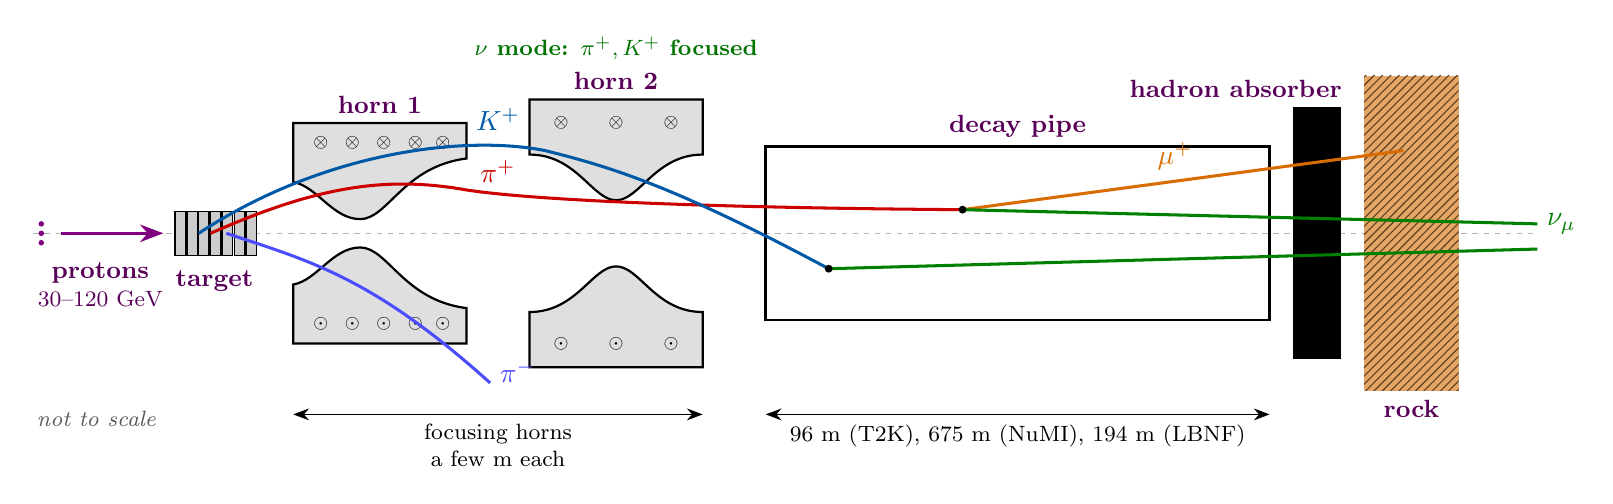
\begin{tikzpicture}[>=Stealth, font=\small,
  cond/.style={fill=gray!25, draw=black, line width=0.8pt},
  dim/.style={<->, line width=0.6pt},
  lab/.style={font=\small\bfseries, text=violet!70!black, align=center},
  track/.style={line width=1.1pt}]

% ---------------- beam axis
\draw[gray!60, dash pattern=on 2pt off 2pt] (-0.5,0) -- (18.6,0);

% ---------------- protons
\foreach \y in {-0.12,0,0.12} \fill[violet] (-0.4,\y) circle (0.035);
\draw[->, violet, line width=1.2pt] (-0.15,0) -- (1.15,0);
\node[lab, below] at (0.35,-0.25) {protons\\[-1pt]\footnotesize\mdseries 30--120 GeV};

% ---------------- target (segmented graphite)
\foreach \i in {0,...,6} \draw[fill=gray!40, line width=0.5pt] (1.3+0.15*\i,-0.28) rectangle ++(0.13,0.56);
\node[lab, below] at (1.8,-0.35) {target};

% ---------------- horn 1 (x = 2.8 ... 5.0)
\draw[cond] (2.8,1.4) -- (5.0,1.4) -- (5.0,0.95) .. controls (4.2,0.85) and (4.0,0.18) .. (3.65,0.18)
            .. controls (3.3,0.18) and (3.1,0.6) .. (2.8,0.65) -- cycle;
\draw[cond] (2.8,-1.4) -- (5.0,-1.4) -- (5.0,-0.95) .. controls (4.2,-0.85) and (4.0,-0.18) .. (3.65,-0.18)
            .. controls (3.3,-0.18) and (3.1,-0.6) .. (2.8,-0.65) -- cycle;
\foreach \x in {3.15,3.55,3.95,4.35,4.7} \node[scale=0.75] at (\x,1.15) {$\otimes$};
\foreach \x in {3.15,3.55,3.95,4.35,4.7} \node[scale=0.75] at (\x,-1.15) {$\odot$};
\node[lab, above] at (3.9,1.4) {horn 1};

% ---------------- horn 2 (x = 5.8 ... 8.0)
\draw[cond] (5.8,1.7) -- (8.0,1.7) -- (8.0,1.0) .. controls (7.4,1.0) and (7.2,0.42) .. (6.9,0.42)
            .. controls (6.6,0.42) and (6.4,1.0) .. (5.8,1.0) -- cycle;
\draw[cond] (5.8,-1.7) -- (8.0,-1.7) -- (8.0,-1.0) .. controls (7.4,-1.0) and (7.2,-0.42) .. (6.9,-0.42)
            .. controls (6.6,-0.42) and (6.4,-1.0) .. (5.8,-1.0) -- cycle;
\foreach \x in {6.2,6.9,7.6} \node[scale=0.75] at (\x,1.4) {$\otimes$};
\foreach \x in {6.2,6.9,7.6} \node[scale=0.75] at (\x,-1.4) {$\odot$};
\node[lab, above] at (6.9,1.7) {horn 2};
\node[font=\footnotesize\bfseries, text=green!45!black] at (6.9,2.35) {$\nu$ mode: $\pi^+,K^+$ focused};

% ---------------- decay pipe
\draw[line width=1pt] (8.8,-1.1) rectangle (15.2,1.1);
\node[lab, above] at (12.0,1.1) {decay pipe};

% ---------------- absorber and rock
\fill[black] (15.5,-1.6) rectangle (16.1,1.6);
\node[lab, above left, xshift=4pt] at (16.1,1.6) {hadron absorber};
\fill[brown!60!orange!70] (16.4,-2.0) rectangle (17.6,2.0);
\fill[pattern=north east lines, pattern color=brown!50!black] (16.4,-2.0) rectangle (17.6,2.0);
\node[lab, below] at (17.0,-2.0) {rock};

% ---------------- tracks
% pi+ : focused, decays in the pipe
\draw[track, red!80!black] (1.75,0) .. controls (3.0,0.55) and (3.9,0.75) .. (5.0,0.55)
      .. controls (6.0,0.4) and (8.5,0.32) .. (11.3,0.3);
\node[red!80!black, font=\normalsize] at (5.4,0.78) {$\pi^+$};
% mu+ from pi+ decay, stops in the rock
\draw[track, orange!85!black] (11.3,0.3) -- (16.9,1.05);
\node[orange!85!black, font=\normalsize] at (14.0,0.98) {$\mu^+$};
% nu_mu from pi+ decay
\draw[track, green!50!black] (11.3,0.3) -- (18.6,0.12);
\node[green!50!black, font=\normalsize, right] at (18.6,0.12) {$\nu_\mu$};
% K+ : wide angle, focused by horn 2, decays
\draw[track, teal!70!blue] (1.6,0) .. controls (3.2,1.05) and (5.0,1.25) .. (6.0,1.05)
      .. controls (6.8,0.85) and (7.6,0.62) .. (9.6,-0.45);
\node[teal!70!blue, font=\normalsize] at (5.4,1.45) {$K^+$};
\draw[track, green!50!black] (9.6,-0.45) -- (18.6,-0.2);
% pi- : defocused
\draw[track, blue!70] (1.95,0) .. controls (3.0,-0.35) and (3.8,-0.55) .. (5.3,-1.9);
\node[blue!70, font=\normalsize] at (5.65,-1.75) {$\pi^-$};
% decay vertices
\fill (11.3,0.3) circle (0.05); \fill (9.6,-0.45) circle (0.05);

% ---------------- dimensions
\draw[dim] (2.8,-2.3) -- (8.0,-2.3) node[midway, below, align=center, font=\footnotesize] {focusing horns\\ a few m each};
\draw[dim] (8.8,-2.3) -- (15.2,-2.3) node[midway, below, align=center, font=\footnotesize]
      {96 m (T2K), 675 m (NuMI), 194 m (LBNF)};
\node[font=\footnotesize\itshape, gray!70!black] at (0.3,-2.35) {not to scale};
\end{tikzpicture}
\end{document}
